\documentclass[times, utf8, zavrsni,numeric,pstricks]{fer}


\graphicspath{{lib/pics/}} %Setting the graphicspath

\definecolor{codegreen}{rgb}{0,0.6,0}
\definecolor{codegray}{rgb}{0.5,0.5,0.5}
\definecolor{codepurple}{rgb}{0.58,0,0.82}
\definecolor{backcolour}{rgb}{0.95,0.95,0.92}
\lstdefinestyle{mystyle}{
    backgroundcolor=\color{backcolour},   
    commentstyle=\color{codegreen},
    keywordstyle=\color{magenta},
    numberstyle=\tiny\color{codegray},
    stringstyle=\color{codepurple},
    basicstyle=\ttfamily\footnotesize,
    breakatwhitespace=false,         
    breaklines=true,                 
    captionpos=b,
    keepspaces=true,                 
    showspaces=false,                
    showstringspaces=false,
    showtabs=false,                  
    tabsize=4  
}

\lstset{style=mystyle}

\begin{document}

% TODO: Navedite broj rada.
\thesisnumber{000}

% TODO: Navedite naslov rada.
\title{Prepoznavanje emocija iz izraza lica pomoću strojnog učenja}

% TODO: Navedite vaše ime i prezime.
\author{Matej Ciglenečki}

\maketitle

% Ispis stranice s napomenom o umetanju izvornika rada. Uklonite naredbu \izvornik ako želite izbaciti tu stranicu.
\izvornik

% Dodavanje zahvale ili prazne stranice. Ako ne želite dodati zahvalu, naredbu ostavite radi prazne stranice.
\zahvala{}

\tableofcontents

\chapter{Uvod}
**Poreba za prepoznavanjem emocija**
**što emocije govore**
**gdje se koristi prepozavanje emocija**
**korištena metoda za klasifikaciju emcoija**


%Prijenosnim učenjem moguće je istrenirani model koji može klasificirati ljudske emocije uz određenu točnost, ovisno o pristupu kojeg koristimo prilikom odabira skupa podataka pomoću kojeg treniramo model.
%
%Odabrani skup podataka Cohn-Kanade koji sadrži sekvence slika ljudskih emocija i njihove označene emocije. Prije samog treniranja potrebno je procesirati i urediti podatke te stvoriti jedinku svake slike koja u sebi ima sve potrebne labele nužne za što bolje stvoren model. To je uređen par (sadržaj slike, emocija, FACS podatak). Pošto za pojedinu sekvencu znamo samo o kojoj se emociji radi potrebno je linearno sklairati neutralnu emociju i emociju o kojoj se radi tako da svaka slika uistinu reprezentira o kojoj se kombinacija emocija radi.



\chapter{Podatkovni skup}
\section{Uvod}
Podatkovni skup sastavni je dio u izvedbi treniranja modela. Treniranje se svodi na ulazne i izlazne podatke gdje su ulazni podaci podskup podatkovnog skupa. Korišteni podatkovni skupovi su Cohn-Kanade (CK) i skup slika preuzetih sa Google-a na temelju ključne riječi. Podatkovni skup dijelimo na dva djela. Skup za treniranje i skup za testiranje. Svi podaci koji su u skupu za treniranje iskorištavaju se za treniranje i optimiziranje odabranog modela dok se skup za testiranje koristi samo za evaluaciju točnosti treniranog modela. 80\% nasumičnih slika odabrane su za treniranje a ostalih 20\% koristi se za evaluaciju.

\section{Extended Cohn-Kanade podatkovni skup}

Cohn-Kanade podatkovni skup sastoji se od 593 sekvenci slika od 123 subjekta (osoba). Pojedina sekvenca sastoji se od 10 do 60 slika. Početna slika u sekvenci je neutralna emocija dok je zadnja slika vrhunac izraza emocije. Subjekti na slikama imaju od 18 do 50 godina, 69\% su žene, 81\% euro-Amerikanci i 6\% su subjekti ostalih rase. Rezolucija pojedine slike iznosi 640x480 ili 640x490 piksela u 8-bitnom crno-bijelom ili 24 bitnom puno-bojnom formatu\cite{ck}. TODO: primjer slike CK+ dataseta

\section{Ručno generirani podatkovni skup}
Slike CK+ podatkovnog skupa slikane su u istom okruženju (ista prostorija u kojoj se slikaju subjekti, ista kamera, slična svjetlina slike...). Nedostatak raznolikosti među slikama stvara potrebu za uvođenjem apstraktnijih slika ljudskih lica ne bi li model klasificirao emocije ljudskih lica koja nisu slična samo CK+ podatkovnom skupu. Zbog toga se uvodi podatkovni skup Google slika. Google omogućuje pretraživanje slika po zadanom upitu te dodatnim parametrima koji olakšavaju pronalaženje ljudskog lica koji predstavlja određenu emociju. Npr. pronalazak ljudskih lica koji iskazuju tužnu emociju mogao bi biti "sad human face" sa tipom Google slike "lice". Rezultati tog upita prikazani su na slici \ref{pic:google_search_sad}.

\begin{figure}[H]
	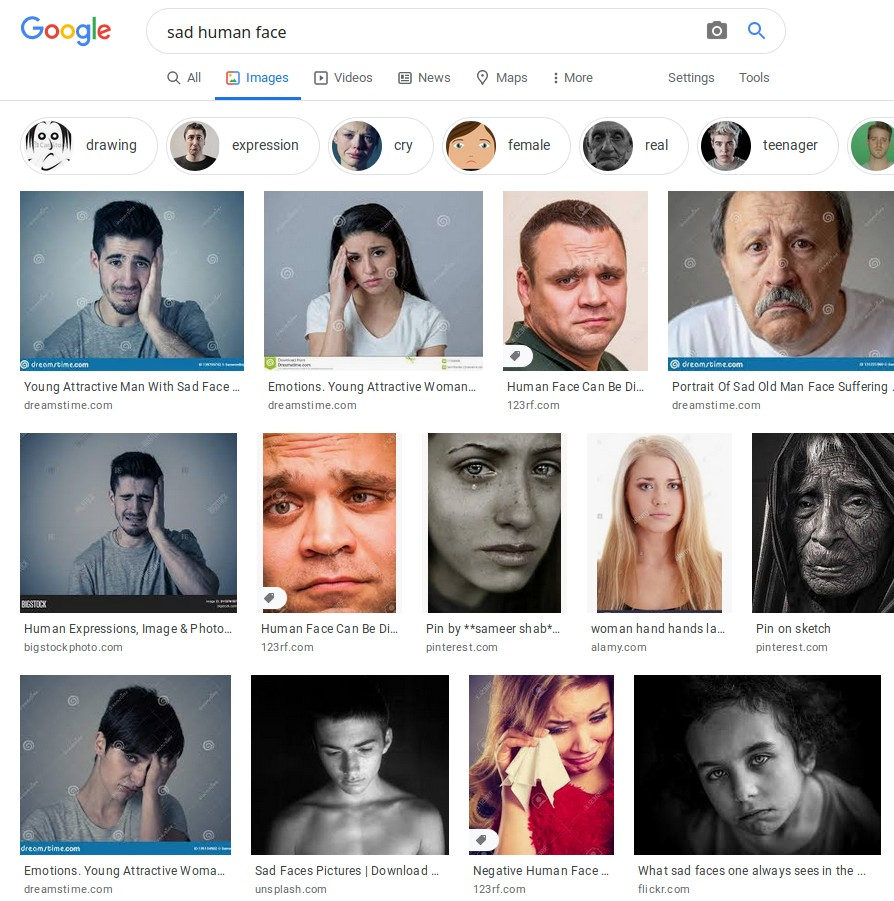
\includegraphics[width=\linewidth]{2020-06-08-22-16-22.jpeg}
	\caption{Rezultati Google upita "sad human face"}
	\label{pic:google_search_sad}
\end{figure}

Rezultati ovog upita su slike veće raznolikosti (različit scenarij i drugačiji kut gledanja) što pridonosi apstrakciji emocije u ukupnom podatkovnom skupu. Dobivene slike ne odgovaraju uvijek nužno zadanom upitu zbog čega je potrebno dodatno provjeriti valjanost pojedine slike. Proces filtriranja objašnjen je u poglavlju \ref{google_npy_filter}


\section{Priprema podatkovnih skupova}
\subsection{Priprema Cohn-Kanade podatkovnog skupa}
\subsubsection{Struktura podataka}

Dijelovi podatkovnog skupa značajni za treniranje dijele se na direktorij sekvence i emocije. Svaki subjekt (npr. S005) ima svoj direktoriji u kojem se nalaze pod direktoriji za emociju koju je subjekt odglumio (npr. 001, 002...) a u njemu se nalaze sekvence. Za 327 sekvenca postoji odgovarajuća emocija koja je definirana samo za krajnju sliku sekvence i njezina putanja je definirana jednako kao i za sekvencu.

\pagebreak

\begin{figure}[H]
\centering
\begin{Verbatim}[fontsize=\small]
├── emotions
│   ├── S005
│   │   └── 001
│   │       └── S005_001_00000011_emotion.txt
│   │       	└── "3.0000000e+00"
│   ├── S010
│   │   ├── 001
│   │   ├── 002
│   │   │   └── S010_002_00000014_emotion.txt
│   │   │   	└── "4.0000000e+00"
│   │   └── ...
│   └── ...
└── images
    ├── S005
    │   └── 001
    │       ├── S005_001_00000001.png
    │       ├── ...
    │       └── S005_001_00000011.png
    ├── S010
    │   ├── 001
    │   │   ├── S010_001_00000001.png
    │   │   ├── ...
    │   │   └── S010_001_00000013.png
    │   ├── 002
    │   │   ├── S010_002_00000001.png
    │   │   ├── ...
    │   │   └── S010_002_00000014.png
    │   └── ...
    └── ...

\end{Verbatim}
\caption{Struktura podataka CK+ podatkovnog skupa}
\label{cb:npy_tree}
\end{figure}

\subsubsection{Obrada podataka}
Jedina slika u sekvenci za koju je definirana emocija je zadnja slika, što znači da je potrebno je potrebno odrediti vektor emocije ostalih slika u sekvenci na temelju krajnje vrijednosti emocije. Emocija za pojedinu sliku definirana je kao red emocija. Svaki indeks reda predstavlja emociju kojih ima kojih ima 8. Indeks pojedine emocije definiran je na slici \ref{cb:emo_declare} a vrijednost na indeksu predstavlja intenzitet emocije

\begin{figure}[H]
\centering
\begin{Verbatim}[fontsize=\small]
emocije = {
    1: "neutral",
    2: "anger",
    3: "contempt",
    4: "disgust",
    5: "fear",
    6: "happy",
    7: "sadness",
    8: "surprise",
}
\end{Verbatim}
\caption{Deklaracija emocija}
\label{cb:emo_declare}
\end{figure}

\noindent
Znajući da je emocija za početnu sliku neutralna a za krajnju maksimalna sekvencijska emocija, emocije za ostale slike dodijeljene su linearno na način da se odredi intenzitet neutralne emocije \ref{eq:intensity_neutral} i sekvencijske emocije \ref{eq:intensity_seq} gdje je $n$ ukupan broj slika u sekvenci a $i$ slika kojoj se određuje vektor emocije.

\begin{equation}\label{eq:intensity_neutral}
	p_{n} = \dfrac{i-1}{n-1}	
\end{equation}
\begin{equation}\label{eq:intensity_seq}
\begin{split}
	p_{s} = 1 - p_{n}\\
	p_{s} + p_{n} = 1	
\end{split}
\end{equation}

\subsubsection{Primjer vektora emocije za sekvencu "disgust" koja sadrži 10 slika:}

\begin{figure}[H]
\centering
\begin{tabular}{|c|c|} 
\hline
broj slike & vektor emocije \\
\hline
$i = 1$ & [1.0, 0.0, 0.0, 0.0, 0.0, 0.0, 0.0, 0.0] \\
... & ... \\
$i = 6$ & [0.4, 0.0, 0.0, 0.6, 0.0, 0.0, 0.0, 0.0] \\
... & ... \\
$i = n = 10$ & [0.0, 0.0, 0.0, 1.0, 0.0, 0.0, 0.0, 0.0] \\
$i$ & [$p_n$, 0.0, 0.0, $p_s$, 0.0, 0.0, 0.0, 0.0]  \\
\hline
\end{tabular}
\caption{Vektor emocije za pojedinu pojedinu sliku u sekvneci u CK podatkovnom skupu}
\label{pic:ck_emotion_rise}
\end{figure}



\subsubsection{Spremanje slike i vektora emocije u .npy podatak}\label{self:npy_save}
Za daljnje korištenje svaka slika i njezin vektor emocije će pretvorena u numpy red \cite{numpy_array} i spremljen kao .npy podatak. Prvi element numpy reda je slika a drugi je odgovarajući vektor emocije. Ovime je osigurano da izračun emocija za pojedinu sliku je izračunat samo jedanput što će smanjiti vrijeme potrebno za treniranje. Nakon provođenja transformacije podataka u .npy podatak ukupan broj slika i pripadajućih vektora emocija iznosi 5703. 



\begin{figure}[H]\label{fig:npy_array}
	\begin{subfigure}[b]{0.5\linewidth}
	  	\centering
		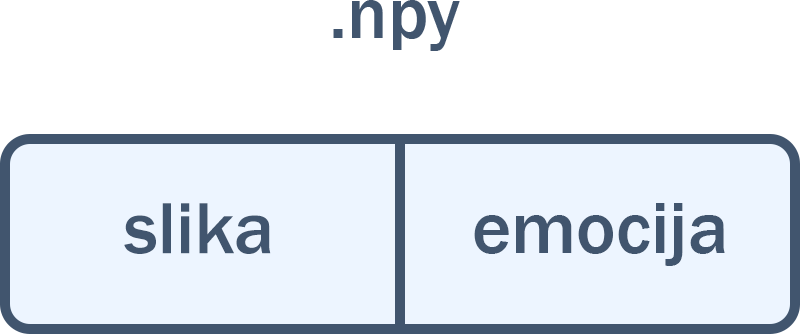
\includegraphics[width=\linewidth]{numpy_slika_emocija.png}
		\caption{Struktura .npy podatka}		
	\end{subfigure}
	\begin{subfigure}[b]{0.5\linewidth}
	  	\centering
		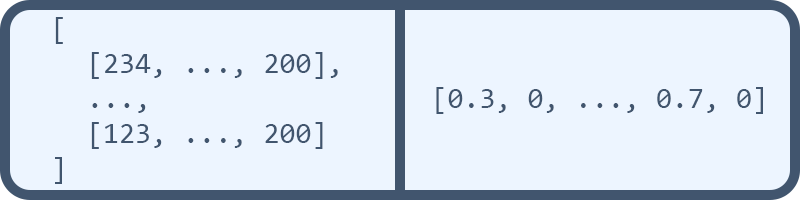
\includegraphics[width=\linewidth]{numpy_imgdata_emo.png}
		\caption{Sadržaj .npy podatka}
	\end{subfigure}	
	\caption{.npy podatak}	
\end{figure}


\subsection{Priprema Google podatkovnog skupa}
\subsubsection{Prikupljeni podaci}
Umjesto preuzimanja jedne po jedne slike korištena je google-images-download skripta \cite{google-images-download} koja preuzima sve moguće slike na temelju zadanog upita. Upiti korišteni za pronalaženje odgovarajućih emocija nalaze se na slici \ref{cb:google_queries} a svi su popraćeni dodatnim "Google search" parametrom koji pretražuje slike samo ljudskih lica. Svaka slika spremljena je u direktoriji čije je ime upit koji je bio korišten prilikom preuzimanje te slike. 

\begin{figure}[H]
	\centering
		\begin{Verbatim}[fontsize=\small]
		"sad human face"
		"neutral human face"
		"neutral expression"
		"angry human face"
		"angry expression"
		"contempt"
		"fear human face"
		"fear expression"
		"surprise human face"
		"surprise expression"
		"disgusted human face"
		"disgust expression"
		\end{Verbatim}
	\caption{Upiti za preuzimanje ljudskih lica sa Google-a}
	\label{cb:google_queries}
\end{figure}

\noindent
Nakon preuzimanja svih mogućih slika potrebno je ručno proći kroz svaki direktorij svakog upita i izbaciti slike koje ne zadovoljavaju sljedeće uvjete \label{google_npy_filter}

\begin{itemize}
	\item Na slici se nalazi samo jedno ljudsko lice
	\item Na slici se nalazi ljudsko lice čija emocija odgovara upitu pomoću kojeg je slika preuzeta
	\item Veličina slike je manja od 20MB
	\item Rezolucija slike je veća od 20px po duljini i visini
	\item Slika nije duplikat prethodno viđene slike
	\item Slika nije dio CK+ podatkovnog skupa
\end{itemize}
Uklanjanjem slika koje ne zadovoljavaju bilo koje od navedenih uvjeta dobiven ukupan broj slika povoljnih za treniranje iznosi 3160 a njihova ukupna veličina je 2,3GB.

\subsubsection{Struktura podataka}
Nakon filtriranja slika nepogodnih za treniranje potrebno je objediniti upite čiji su rezultati ljudska lica efektivno istih emocija. Primjer takva dva upita su "neutral human face" i "neutral expression". Nakon objedinjavanja rezultata upita i preimenovanja direktorija stvorena je struktura podataka dana na slici \ref{cb:google_file_structure}


\begin{figure}[H]
\centering
\begin{Verbatim}[fontsize=\small]
├── neutral
│   ├── 1.57053528-man-head-shot.png
│   ├── 2.Face_of_SpooSpa.png
│   ├── 3.main-1-low-res-4a61d.png
│   └── ...
├── anger
│   ├── 1.57053528-man-head-shot.png
│   └── ...
├── contempt
│   └── ...
├── disgust
│   └── ...
├── fear
│   └── ...
├── happy
│   └── ...
├── sadness
│   └── ...
└── surprise
    └── ...
\end{Verbatim}
\caption{Struktura podataka Google podatkovnog skupa}
\label{cb:google_file_structure}
\end{figure}

\subsubsection{Obrada podataka}
Obrada Google podatkovnog skupa bit će manje zahtjevna od CK+ podatkovnog skupa zbog toga što će se vektor emocije za pojedinu sliku odrediti samo na temelju upita korištenog za preuzimanje slike. Rezultat svakog vektora emocije bit će vektor dobiven metodom "One hot encoding". "One hot encoding" je metoda dodjele binarne vrijednosti za kategoriju u koju neki uzorak pripada ili ne pripada\cite{one_hot_encoding}. Ovom metodom uzorak (slika) može pripadati samo jednoj kategoriji (emocija). Slika koja pripada određenoj emociji za tu će emociju imati vrijednost 1 a za sve ostale 0. Na slici \ref{pic:google_emotion_emo_vector} prva kolumna označava ime direktorija u kojem se slike nalaze, druga kolumna predstavlja vektor emocije koje će slike u direktoriju poprimiti.

\begin{figure}[H]
\centering
\begin{tabular}{|c|c|} 
\hline
emocija (ime direktorija) & vektor emocije \\
\hline
neutral & [1,0,0,0,0,0,0,0] \\
anger	& [0,1,0,0,0,0,0,0] \\
contempt & [0,0,1,0,0,0,0,0] \\
disgust & [0,0,0,1,0,0,0,0]\\
fear  & [0,0,0,0,1,0,0,0]\\
happy & [0,0,0,0,0,1,0,0]\\
sadness & [0,0,0,0,0,0,1,0]\\
surprise & [0,0,0,0,0,0,0,1]\\
\hline
\end{tabular}
\caption{Vektor emocije za pojedinu emociju u Google podatkovnom skupu}
\label{pic:google_emotion_emo_vector}
\end{figure}

\subsubsection{Spremanje slike i vektora emocije u .npy podatak}
Nakon dodjele vektora emocije za pojedinu sliku potrebno je pretvoriti sliku i vektor emocije u .npy podatak. Kako se radi o slici i vektoru emocije, postupak pretvorbe slike i vektora emocije u pojedinačni .npy podatak jednak je kao i kod CK+ podatkovnog skupa definiranom u poglavlju \ref{self:npy_save}.


\subsection{Objedinjavanje podatkovnih skupova}
Nakon obrade CK+ i Google podatkovnog skupa svi .npy podaci bit će spremljeni u direktoriji "ck" ili "Google" ovisno o tome iz kojeg je podatkovnog skupa slika dobivena. Struktura svih .npy podataka prikazana je na slici \ref{pic:npy_structure}. Ovom strukturom moguće je definirati udio svakog podatkovnog skupa koji će biti korišten za treniranje modela.


\begin{figure}[H]
\centering
\begin{Verbatim}[fontsize=\small]
numpy
├── ck
│   ├── slika_i_emocija_0001.npy
│   ├── ...
│   └── slika_i_emocija_5703.npy
└── google
    ├── slika_i_emocija_0001.npy
    ├── ...
    └── slika_i_emocija_3160.npy
    

\end{Verbatim}
\caption{Struktura .npy podataka}
\label{pic:npy_structure}
\end{figure}



\chapter{Treniranje}
Treniranje je proces u kojem model postupno mijenja svoje parametre ne bi li došao do idealnih parametara, čime bi model optimalno služio onome čemu je namijenjen. U slučaju klasifikacije za treniranje je potrebno imati skup podataka nad kojim će se provoditi treniranje i labele tih podataka koje govore klasu podataka. U slučaju klasifikacije emocija, skup podataka nad kojim se trenira su slike ljudskih lica dok je klasa emocija koja je prikazana na pojedinoj sliku. Kad treniranje započne, u model se pošalju podaci za koje model pokušava predvidjeti koje su klase ubačeni podaci. Nakon toga potrebno je usporediti predviđanja klasa koje je stvorio model sa pravim klasa. Pogrešku koju je model napravio prilikom predviđanja potrebno je javiti modelu ne bi li ispravio parametre. Mijenjanjem modela parametra model postaje sve bolji za predviđanje predviđanje rezultata na skupu za treniranje. Bitno je naglasiti da daljnjim treniranjem model ne postaje bolji za općeniti slučaj predviđanja. Treniranjem model se prilagođava podatkovnom skupu za treniranje. Podatkovni skup za treniranje je podskup svih podataka za koje je model namijenjen a to znači da skup za treniranje nije nužno najbolja mjera općenitog slučaja za podatke. 


Treniranje modela nakon određenog trenutka može pogoršati sposobnost modela da predviđa klase na općenitom slučaju. Uzrok toga je što treniranjem nakon točke TODO:NAME model ima veću točnost na skupu za treniranje ali točnost na općenitim, neviđenim slučajevima postaje sve manja. Zbog toga je potrebno pronaći optimalan trenutak u kojem treba prekinuti treniranje modela. Prekidanje treniranja modela nije moguće odrediti pomoću točnosti modela na skupu za treniranje jer ta točnost neprestano raste daljnjim treniranjem. Zbog toga je potrebno uvesti validacijski skup koji neće biti korišten prilikom treniranja. Validacijski skup o tom slučaju igra ulogu neviđenih podataka nad kojima se mjeri točnost. Prilikom treniranja točnost nad validacijskim skupom će rasti do točke TODO:ANME. U tom trenutku točnost nad validacijskim skupom će biti maksimalna a daljnjim treniranjem točnost će se smanjivati jer model postaje previše prilagođen skupu za treniranje \textit{(engl. overfitting)}. 

TODO: slika - skup podataka  
**načini treniranja**

\section{Duboke neuronske mreže za analizu slika}
\subsection{Neuron}
Neuron je osnovni dio neuronske mreže. Svaki neuron na svoj ulaz prima vektor $x$ vrijednosti za koje neuron predviđa $\hat{y}$ izlaz. Skup $x$ vrijednosti je također pomnožen sa vektorom $w$ koji predstavlja težine \textit{(engl. weights)} i zbrojen sa vrijednošću $b$ koja predstavlja sklonost \textit{(engl. bias)}


\begin{equation}\label{eq:neuron}
	z=w_1x_1+w_2x_2+...+w_nx_n=w^{T} \cdot x
\end{equation}

\begin{equation}\label{eq:neuron}
	\hat{y} = g(z)
\end{equation}

\subsubsection{Aktivacijska funckija}

Nakon zbrajanja kroz neuron izlaz je potrebno provesti kroz aktivacijsku funkciju određuje koliko je signal tog neurona bio zastupljen u ukupnom izlazu, tj. koliko je "aktiviran". Cilj koji se postiže tom funkcijom je da ukupan izlaz neurona bude između vrijednosti 0 i 1. Dakle to su funkcije za koje vrijedi \ref{eq:activation_fun_general}. Primjer takvih funckija je sigmoid prikazan na slici \ref{fig:sigmoid} i ispravljač \textit{(ReLU - engl. Rectifier)} prikazan na slici \ref{fig:relu}

\begin{equation}\label{eq:activation_fun_general}
	f:\mathbb{R} \rightarrow [0,1]
\end{equation}

\begin{figure}[H]
	\centering
		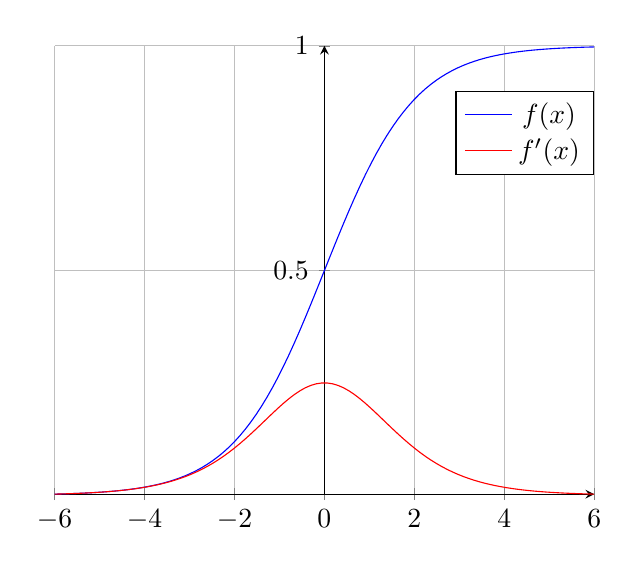
\begin{tikzpicture}[declare function={
			sigma(\x)=1/(1+exp(-\x));
			sigmader(\x)=sigma(\x)*(1-sigma(\x));
			},scale=1]
			
			\begin{axis}%
			[
			    grid=major,     
			    xmin=-6,
			    xmax=6,
			    axis x line=bottom,
			    ymax=1,
			    axis y line=middle,
			    ytick={0,.5,1},
			    samples=100,
			    domain=-6:6,
			    legend style={at={(1,0.9)}}     
			]
			    \addplot[blue,mark=none]   (x,{sigma(x)});
			    \addplot[red,mark=none]   (x,{sigmader(x)});
			    \legend{$f(x)$,$f'(x)$}
			\end{axis}
			\end{tikzpicture}
		\caption{Sigmoid}	
		\label{fig:sigmoid}	
\end{figure}		

\begin{figure}[H]
	\centering
		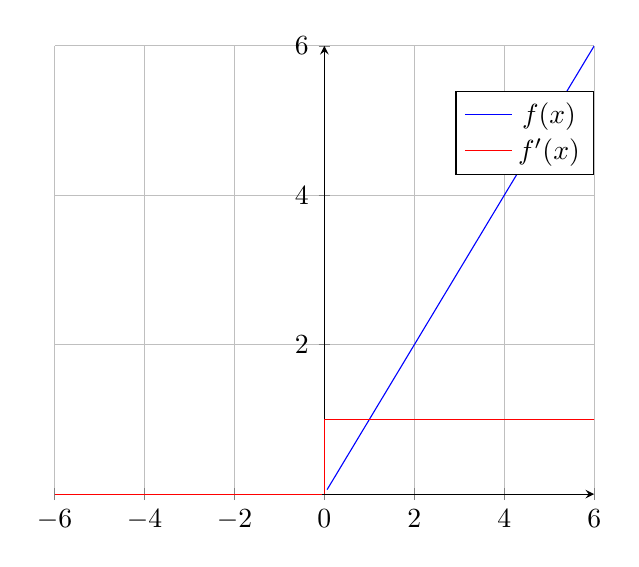
\begin{tikzpicture}[declare function={
			linear(\x)=\x;
			linearder(\x)=\x;
			},scale=1]
			
			\begin{axis}%
			[
			    grid=major,     
			    xmin=-6,
			    xmax=6,
			    axis x line=bottom,
			    ymax=6,
			    axis y line=middle,
			    samples=100,
			    domain=-6:6,
			    legend style={at={(1,0.9)}}     
			]	
			   \addplot[blue, restrict expr to domain={}{0:inf}]  (x,{linear(x)});
				\addplot[blue,  forget plot, restrict expr to domain={}{-inf:0}]  (x,0);
				\addplot[red, restrict expr to domain={}{-inf:0}]  (x,0);
				\addplot[red, const plot]  coordinates {(-inf,0) (0,0) (0,1) (100,1)};
			   \legend{$f(x)$,$f'(x)$}
			\end{axis}
			\end{tikzpicture}
		\caption{ReLU}
		\label{fig:relu}
\end{figure}

\subsection{Sloj neurona}




**općenito**2
**problem treniranja dubokih mreža**	
**gradient degradation problem**


\subsection{Rezidualna neuronska mreža}

\subsection{ResNet 50}
**probleme koje riješava**

**kako funckionira**

\subsection{Prijenosno učenje}
**transfered learning**

**zasto ga koristimo umjesto cijelokupnog treniranja**

**nedostatak labeliranih slika**

\section{Implementacija treniranja u PyTorch-u}
\subsection{Priprema podataka}
\subsubsection{Augmentacija slika}
\subsubsection{Transformacija podataka}


\subsection{ResNet 50}
\subsection{Adam optimizator}
\subsection{Funckija gubitka}
\subsubsection{križni entropijski gubitak}
\subsection{Treniranje}

\chapter{Testiranje/evaluacija}

\chapter{Zaključak}
Zaključak.

\bibliography{literatura}
\bibliographystyle{fer}

\begin{sazetak}
Sažetak na hrvatskom jeziku.

\kljucnerijeci{Ključne riječi, odvojene zarezima.}
\end{sazetak}



% TODO: Navedite naslov na engleskom jeziku.
\engtitle{Title}
\begin{abstract}
Abstract.

\keywords{Keywords.}
\end{abstract}

\end{document}
